\documentclass[a4paper, 10pt]{article}

\usepackage[utf8]{inputenc}
\usepackage{fancyhdr}
\usepackage{pdfpages}
\pagestyle{fancy}
\setlength{\headheight}{24.0pt}

\rfoot{
	\begin{tabular}{r}
		Future User Interfaces\\
	\end{tabular}
}

\lhead{
	\begin{tabular}{l}
		SS 15\\
	\end{tabular}
}

\rhead{
	\begin{tabular}{l}
		Christoph Reinhart, Nicolas Spycher, Raphaël Thuor
	\end{tabular}
}

\begin{document}

	\title{Library application with gesture- and speech-based interface}
	\maketitle
	
	\begin{tabular}{rl}
		Christoph Reinhart  & christoph.reinhart@students.unibe.ch\\
		Raphaël Tuor  & raphael.tuor@gmail.com\\
		Nicolas Spycher & nicolas.spycher@students.unibe.ch
	\end{tabular}
	
	\newpage	
	\section{The application}
	
	\par{The idea behind the project, was to design and implement a Library Application which can hold the entire catalog of a Library and simplify the search and handling of the books. This would enable a library to display the whole collection of books, even if there isn't enough space on the shelves to display all of them. This system could be placed in the entryway of a library and give the customers the ability to browse the whole catalog even before entering the library itself.}
	\par{The application offers the user the ability to look up books and open them. The search function is programmed as a filter and displays all the available books if no filter is applied. The user is also able to bookmark the books he is interested in which then in a future version could be managed in some kind of user profile with a corresponding user login. Furthermore the applications provides the ability to mark a certain keyword in a opened book and use it as a search term. Other minor functionality includes jumping to a certain page and searching for keywords inside a book.}
	
	
	\section{The interfaces}
	
	\subsection{Gesture and speech}
	
	\par{The first interface is controlled with voice and gesture commands and is implemented using a Kinect device. The interface includes functionality that can be handled only with speech, only with gestures, with speech or gestures and some that can only be controlled using both inputs. Specific information about the commands follows in the next section}
	
	\subsection{Keyboard and mouse}
	
	\par{As a second interface we chose the traditional keyboard and mouse interface. This decision was made due to our main question which we wanted to be able to answer with this project. Our research question was, whether the use of a sophisticated interface can improve usability and productivity of the user or if on the other hand the keyboard and mouse interface is still a better way to go through information.}
	
	
	\section{Functionality}
	
	\par{This section gives an overview over the functionality of the application and positions the multimodal interactions according to the CASE and CARE models. The positioning is marked in brackets in the following format (CASE positioning / CARE positioning). In the future the speech and gesture interface is referred to as the 1st interface whereas the keyboard and mouse interface is referred to as the 2nd interface.}
	
	\subsection{Search}
	
	\subsubsection{1st interface}
	
	\par{If the user wants to search for a book he first has to say 'new search'. Then he can provide a keyword. This part of the interface is not multimodal. The found books are presented to the user with thumbnails of the book covers. To open a certain book the user has to move the mouse over the thumbnail with gestures and can then say the word 'open'  (Alternate/Assignment). The book opens in the application itself.}
	
	\subsubsection{2nd interface}
	
	\par{The user can click in the search field and enter a keyword to search for certain books(Alternate/Assignment). For initiating the actual search he can ether press the search button or press the enter key. This would be Equivalence in the sense of the CARE model. To open a book the user clicks on the thumbnail with the mouse. (-/Assignment).}
	
	\subsection{Browsing book}
	
	\subsubsection{1st interface}
	
	\par{Once a book is open the user is presented with a couple of functionality. He can either swipe vertically to go from page to page or continuously scroll through the document by horizontally swiping (-/Complementarity). If he wants to jump to a certain page he can do so by saying 'jump to' and providing a page number by speech input (-/Assignment). The user is also able to search for a keyword in the book. He can do so by saying 'search for' and providing a keyword by speech input (-/Assignment). While in the search mode the user is able to go to the next occurrence of the word by either swiping vertically or saying the word 'next' or 'previous' (-/Equivalence).}
	\par{Furthermore the user can move the cursor over a word in the document with gestures and then say the word 'highlight' to highlight a certain word (Alternate/Assignment). After that he can search for this keyword by saying 'search for keyword' (-/Assignment).  }
	
	\subsubsection{2nd interface}
	
	\par{The same functionality is available for the keyboard and mouse interface. To go to the next or previous page or jump to a certain page the user has to use the predefined adobe acrobat reader controls of the application (-/Assignment). To scroll trough the document he can either use his mouse wheel or use the slider of the document viewer on the right side (-/Equivalence). If he wants to search for a word within the document he can either press ctrl+f or look for the functionality in the menu of the document viewer (-/Equivalence). To go to the next occurrence of the word he can use the mouse to click on the arrow buttons or use the keyboard arrow buttons (-/Equivalence).}
	\par{To use a word from the text as keyword the user has to copy the file into the search field and the initiate the search (Alternate/Assignment).}
	
	\subsection{Bookmark}
	
	\subsubsection{1st interface}
	
	\par{The user is also able to bookmark the books he likes to remember. To do so he first has to open a book as described before and then say the words bookmark or unbookmark if he wants to remove the book from his bookmarks (Alternate/Assignment). To get an overview over his bookmarks the user can say the word \"show bookmarks\" (-/Assignment).}
	
	\subsubsection{2nd interface}
	
	\par{For the keyboard and mouse interface this functionality is handled with three buttons for bookmarking, unbookmarking and show bookmarks. The user also hast to open a book first before he can use the buttons (Alternate/Assignment).}
	
	
	\subsection{Evaluation}
	
	\par{To evaluate both user interfaces and answer our research question we chose to do both qualitative and quantitative evaluation. Because of limited time and people we decided to do the evaluation within-group. The questionnaire can be found in the appendix.}
	
	\newpage
	\appendix
	
	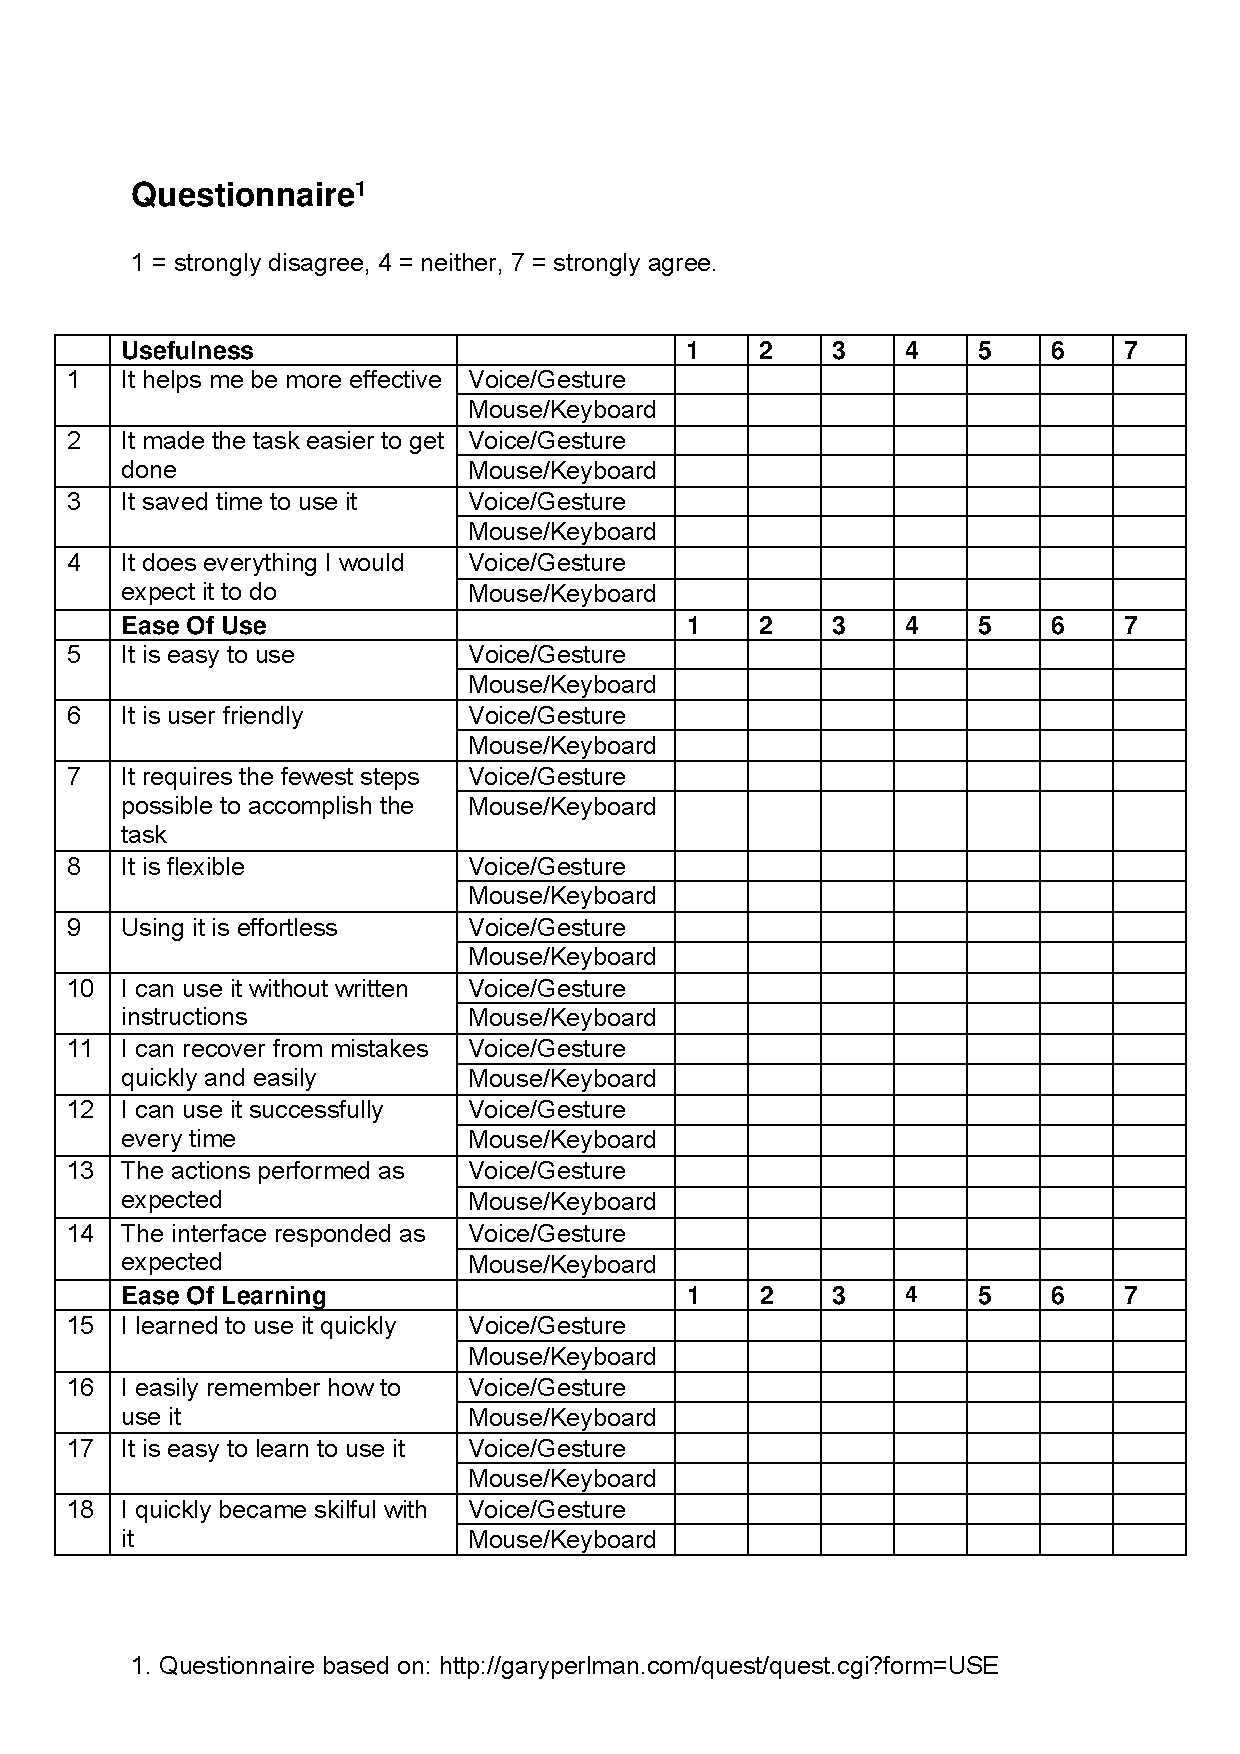
\includepdf[scale=0.8,page=1, pagecommand=\section{Questionnaire}]{questionnaire.pdf}
	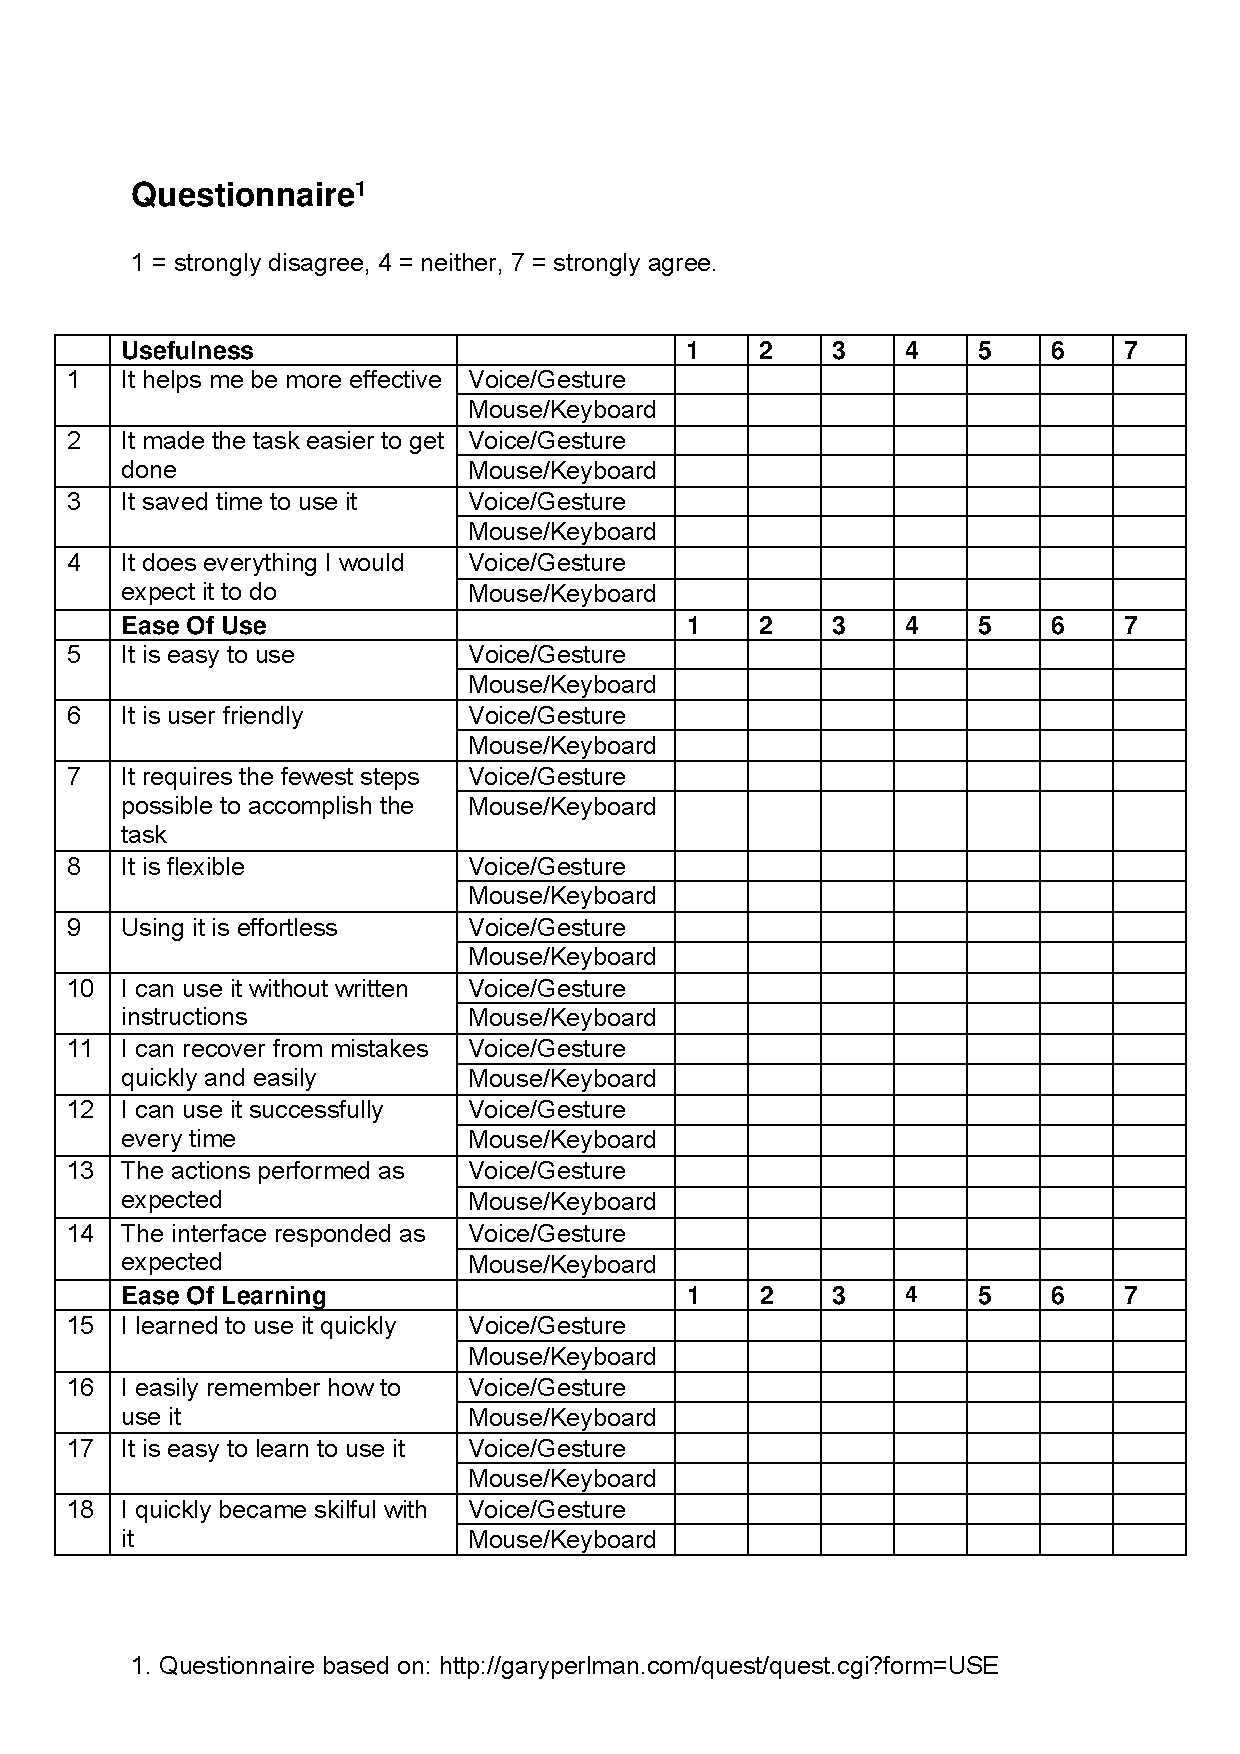
\includepdf[scale=0.8,page=2-, pagecommand={}]{questionnaire.pdf}
	
	
	
	
	
	

\end{document}
